\section{Pushing Heavy Objects: Force Policies for Rigid Body Transport}
\label{sec:pho}

The previous section demonstrated that object-centric force-space policies enable generalizable manipulation of articulated objects whose motion is constrained by joints. This section extends the approach to a complementary class of sustained-contact manipulation: transporting rigid objects along prescribed paths through sustained boundary contact, where the primary challenge is not joint-constrained motion but unknown and varying contact resistance due to object mass and surface friction~\citep{goel2025pho}.

\subsection{Problem Setting}
\label{sec:pho_problem}

We consider a rigid object with planar pose $(c, \theta) \in \Real^2 \times (-\pi, \pi]$ driven by boundary contact forces $f = (F_x, F_y)^\top \in \Real^2$ under a quasi-static regime in which inertial effects are negligible relative to frictional resistance. The object must be transported along a prescribed planar reference path $\Gamma \subset \Real^2$ while maintaining bounded lateral deviation and orientation error over a finite horizon $T$. The object mass $m$ and surface friction coefficient $\mu$ are not assumed known a priori and jointly determine the contact resistance required to initiate and sustain motion.

This setting presents three coupled sub-problems: (1) learning an object-centric path-following policy that outputs boundary forces conditioned on a compact interaction descriptor; (2) inferring the interaction descriptor from onboard sensing, without explicit identification of mass and friction; and (3) physically realizing the desired boundary forces on a robot through compliant control. The decomposition mirrors the structure of FLEX---policy learning, interactive estimation, robot execution---but addresses a fundamentally different object class and interaction regime.

\begin{figure}[t]
    \centering
    
\includegraphics[width=\textwidth]{figures/chapter5/arch.pdf}
    \caption{Architecture of the pushing heavy objects framework. The policy is trained in simulation (top right) using a parameterized MDP conditioned on an interaction descriptor $z$. At deployment (bottom), the robot estimates $z$ through impedance-based force probing and constructs the object-centric state from proprioceptive sensing, then executes the learned boundary forces through compliant impedance control.}
    \label{fig:pho_architecture}
\end{figure}


\subsection{Object-Centric Policy Learning}
\label{sec:pho_policy}

The force policy is learned entirely in simulation, without modeling robot embodiment. Learning is formalized as a parameterized Markov Decision Process:
\[
M(z) = \langle S, A, T_z, R, \gamma \rangle,
\]
where $z \in \mathcal{Z}$ is a task-relevant interaction descriptor sampled once per episode and held fixed during rollout. The state $s_t \in S \subset \Real^6$ is an egocentric, path-relative representation:
\[
s_t = \left( e^\text{lat}_t,\; e^\theta_t,\; v^{\parallel}_t,\; v^{\perp}_t,\; \omega_t,\; z \right),
\]
where $e^\text{lat}_t$ is the signed lateral deviation from the path, $e^\theta_t$ is the orientation error relative to the path tangent, $v^{\parallel}_t$ and $v^{\perp}_t$ are velocity components along the tangent and normal, $\omega_t$ is the angular velocity, and $z \in [0, 1]$ is a normalized contact-resistance scalar encoding the interaction regime.

\begin{figure}[t]
    \centering
    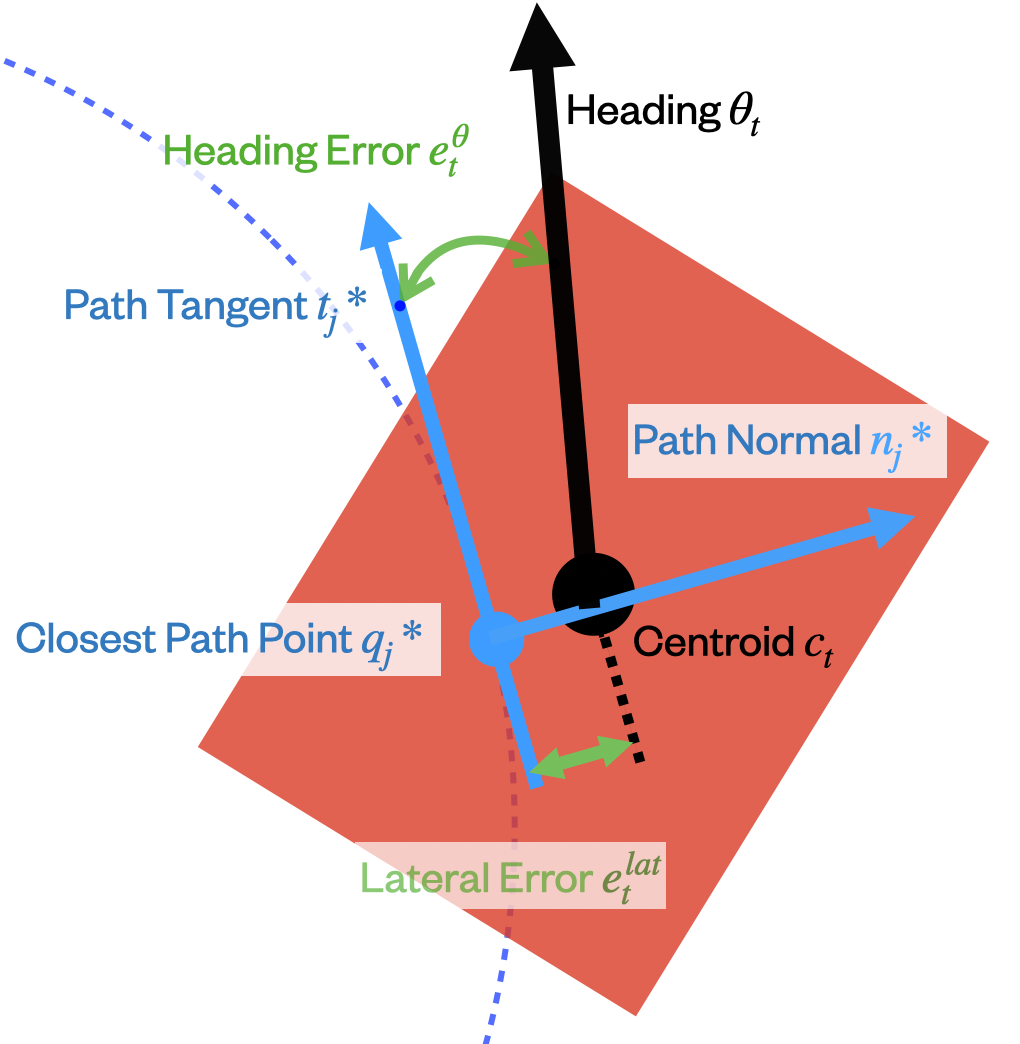
\includegraphics[width=0.55\textwidth]{figures/chapter5/state_description.png}
    \caption{Diagrammatic representation of the state space in the parameterized MDP. The object's pose is represented relative to the reference path through lateral deviation $e^\text{lat}_t$, heading error $e^\theta_t$, and velocity components along the path tangent and normal. The normalized contact-resistance descriptor $z$ conditions the policy on the interaction regime.}
    \label{fig:pho_state}
\end{figure}

The action space $A = \{ f \in \Real^2 \mid \|f\| \leq F_\text{max} \}$ consists of planar boundary forces applied at the contact point, with $F_\text{max} = 200$~N. Object rotation arises implicitly from the lever-arm geometry $\tau = r \times f_t$, without requiring an explicit torque command.

The reward function promotes efficient path tracking through a combination of progress, speed regulation, lateral deviation, orientation alignment, and spin penalties:
\begin{equation}
\label{eq:pho_reward}
R(s_t, f_t, s_{t+1}) = \alpha\, v^{\parallel}_t e^{-\beta |e^\text{lat}_t|} - \lambda\, (v^{\parallel}_t - v_\text{ref})^2 - \kappa\, (e^\text{lat}_t)^2 - \eta\, (e^\theta_t)^2 - \xi\, \omega_t^2 + \delta\, \mathbb{1}\{\text{goal reached}\}.
\end{equation}

The policy is trained using TD3~\citep{fujimoto2018td3} with a segment-based curriculum and domain randomization over mass ($5$--$15$~kg) and friction ($\mu \in [0.4, 0.6]$). During training, the normalized descriptor is computed as $z = \text{clip}(\mu m g / F_\text{max}, 0, 1)$, providing the policy with a compact summary of the interaction regime.


\subsection{Interactive Estimation}
\label{sec:pho_estimation}

At deployment, the robot does not have access to the object's mass or friction coefficient. The interaction descriptor $z$ is estimated through a lightweight impedance-based probing routine that requires only proprioceptive force sensing.

Starting from an established boundary contact, the robot incrementally displaces the impedance controller's equilibrium point along a probe axis while measuring the contact force. As the offset increases, the reaction force rises due to static friction until breakaway occurs. The peak force $f_\text{max}$ prior to breakaway is recorded, and the interaction descriptor is computed as:
\[
z = \text{clip}\left(\frac{f_\text{max}}{F_\text{max}}, 0, 1\right).
\]

The descriptor $z$ approximates the breakaway friction force required to initiate sliding. Under quasi-static planar pushing, this force scales with $\mu m g$, capturing the combined influence of object mass and surface friction without requiring explicit identification of either parameter individually. The scalar $z$ remains fixed for the duration of the episode.

After estimating $z$, the remaining state components are computed at each control step from proprioceptive measurements. The object centroid is recovered from the known contact offset, and geometric errors (lateral deviation, heading error) and kinematic quantities (velocities, angular velocity) are computed relative to the reference path.


\subsection{Robot Execution}
\label{sec:pho_execution}

The learned boundary forces are realized on hardware through compliant impedance control. At each control step, the policy outputs a desired planar force $f_t$, which is converted into a Cartesian displacement command via an admittance-style mapping:
\[
\Delta x_t = \frac{f_t}{K_\text{eff}},
\]
where $K_\text{eff}$ is the effective planar stiffness of the impedance controller. The resulting contact force $F_\text{contact} \approx K_\text{eff}(x_\text{ref} - x) + \zeta \frac{dx}{dt} \approx f_t$, where $\zeta$ is the virtual damping. This compliant execution layer allows small pose deviations to generate interaction forces while preventing excessive contact instability.

The policy operates in object-centric force space; the impedance controller serves only to realize boundary forces through compliant motion, independent of the robot's specific kinematic structure. This separation between force-level decision-making and embodiment-specific control enables zero-shot transfer from simulation to hardware without policy retraining.


\subsection{Experimental Evaluation}
\label{sec:pho_results}

\subsubsection{Simulation Experiments}

Policies were trained in MuJoCo~\citep{todorov2012mujoco} with mass randomized over $[5, 15]$~kg and friction over $[0.4, 0.6]$, using short arc segments from a circular path of radius 1.5~m. Generalization was evaluated under single-parameter out-of-distribution (OOD) shifts.

\paragraph{Parameter generalization.} \Cref{tab:pho_ood} reports tracking performance (centroid-to-path RMSE) under controlled OOD shifts. The fully in-distribution baseline achieves $2.9 \pm 0.4$~cm. Across all OOD conditions---mass, friction, path radius, and box dimensions---RMSE remains within a narrow range of $2.7$--$3.3$~cm, demonstrating stable generalization. Box dimension and path radius variations were introduced only at evaluation time and not included during training.

\begin{table}[t]
\footnotesize
\centering
\begin{tabular}{l c c}
\toprule
Parameter & OOD Low RMSE (cm) & OOD High RMSE (cm) \\
\midrule
Mass      & $3.1 \pm 0.4$ & $3.3 \pm 0.5$ \\
Friction  & $3.3 \pm 0.8$ & $2.8 \pm 0.3$ \\
Path radius & $2.7 \pm 0.3$ & $3.1 \pm 0.4$ \\
Box dimensions & $3.1 \pm 0.6$ & $2.8 \pm 0.2$ \\
\bottomrule
\end{tabular}
\caption{Parameter generalization for pushing heavy objects. Centroid-to-path RMSE (cm) under single-parameter out-of-distribution shifts. The in-distribution baseline achieves $2.9 \pm 0.4$~cm. Performance remains stable across all OOD conditions.}
\label{tab:pho_ood}
\end{table}


\paragraph{Path generalization.} \Cref{tab:pho_paths} evaluates generalization to novel path geometries with physical parameters kept in-distribution. Performance degrades gradually as curvature increases: 60° and 120° arcs remain close to baseline ($2.2$--$2.8$~cm), while S-shaped and sinusoidal paths---which introduce curvature sign reversals absent from training---show higher RMSE ($9$--$10$~cm). Even in the most challenging cases, the deviation remains well below one-fifth of the object width, indicating bounded transport despite the distribution shift.

\begin{table}[t]
\footnotesize
\centering
\begin{tabular}{l c}
\toprule
Path geometry & RMSE (cm) \\
\midrule
Arc 60°   & $2.2 \pm 0.3$ \\
Arc 120°  & $2.8 \pm 0.3$ \\
Arc 180°  & $5.2 \pm 2.2$ \\
S-Path    & $9.0 \pm 6.2$ \\
Sine-Wave & $10.1 \pm 6.6$ \\
\bottomrule
\end{tabular}
\caption{Path generalization for pushing heavy objects. RMSE (cm) under novel path geometries with in-distribution physical parameters. Performance degrades gracefully with increasing curvature complexity.}
\label{tab:pho_paths}
\end{table}


\paragraph{Interaction descriptor ablation.} \Cref{tab:pho_ablation} presents an ablation study evaluating the role of the normalized contact-resistance descriptor $z$. Removing the descriptor ($z = 0$) increases tracking error by 45\%, while setting $z = 1$ produces an order-of-magnitude increase in RMSE with high variance. Replacing the descriptor with its in-distribution mean ($\mathbb{E}[z] = 0.245$) yields nearly identical performance to the full system, suggesting that the policy uses $z$ as a coarse regime indicator rather than a precise estimate.

\begin{table}[t]
\footnotesize
\centering
\begin{tabular}{l c c}
\toprule
Descriptor setting & $z$ value & RMSE (cm) \\
\midrule
Estimated (full system) & $0.10$--$0.44$ & $2.87 \pm 0.35$ \\
Mean value              & $0.245$         & $2.79 \pm 0.40$ \\
Fixed at minimum        & $0$             & $4.16 \pm 0.77$ \\
Fixed at maximum        & $1$             & $34.15 \pm 33.50$ \\
\bottomrule
\end{tabular}
\caption{Ablation study for the interaction descriptor $z$. The descriptor provides meaningful conditioning for the learned policy; removing it significantly degrades performance.}
\label{tab:pho_ablation}
\end{table}



\begin{figure}[t]
    \centering
    \begin{subfigure}[t]{0.48\textwidth}
        \centering
        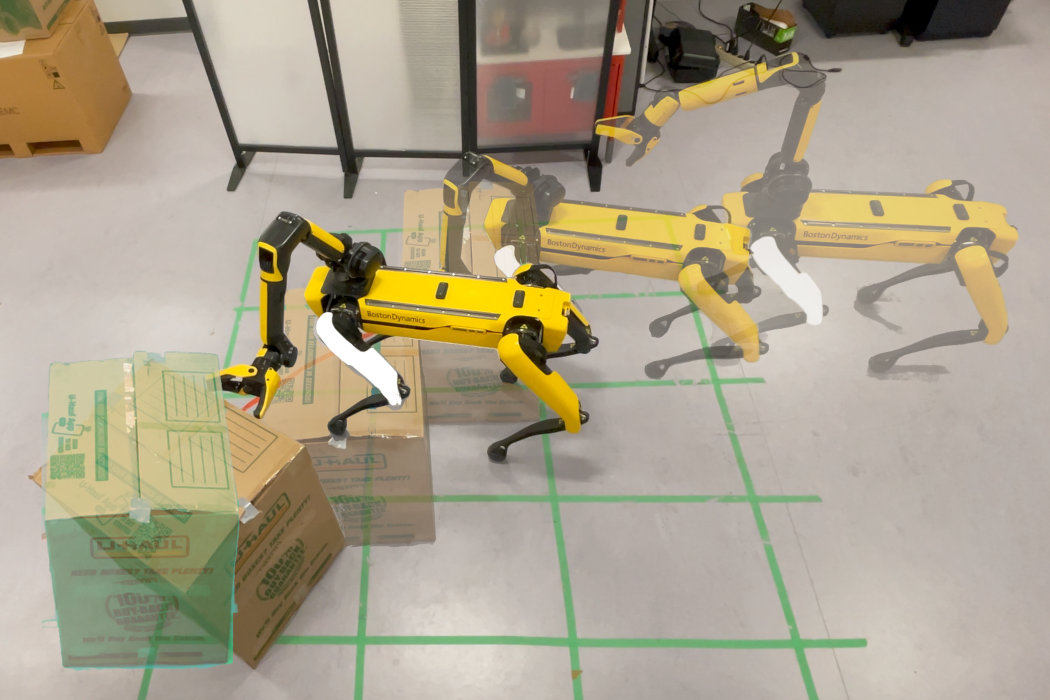
\includegraphics[width=\textwidth]{figures/chapter5/8pt8kg-policy.jpg}
        \caption{Policy, 8.8\,kg}
    \end{subfigure}
    \hfill
    \begin{subfigure}[t]{0.48\textwidth}
        \centering
        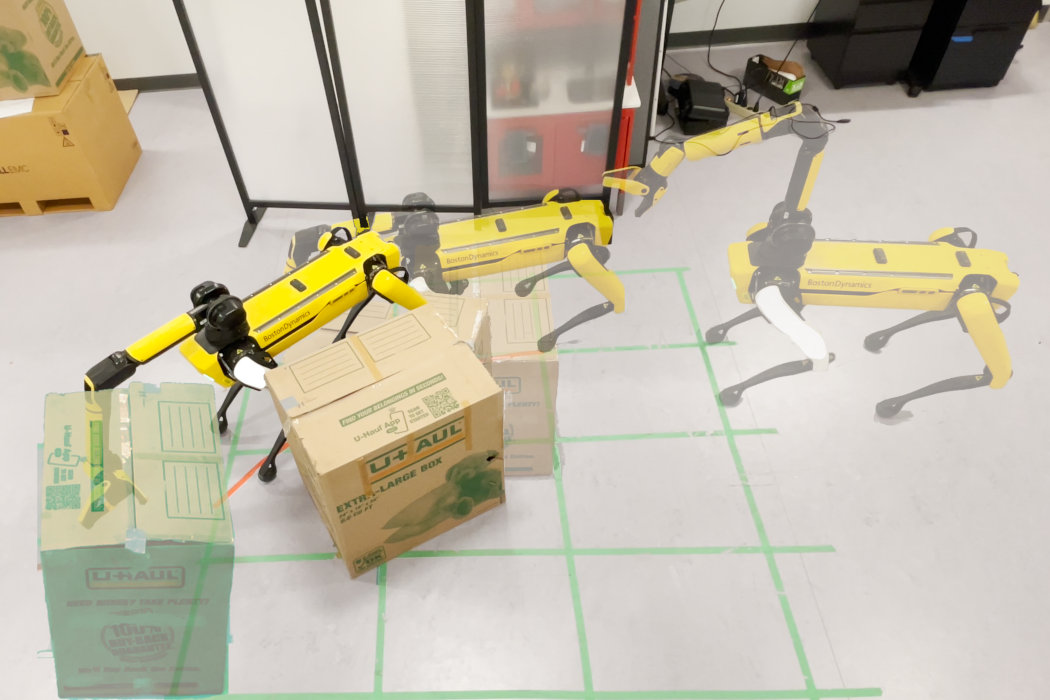
\includegraphics[width=\textwidth]{figures/chapter5/8pt8kg-baseline.jpg}
        \caption{Baseline, 8.8\,kg}
    \end{subfigure}
    \\[6pt]
    \begin{subfigure}[t]{0.48\textwidth}
        \centering
        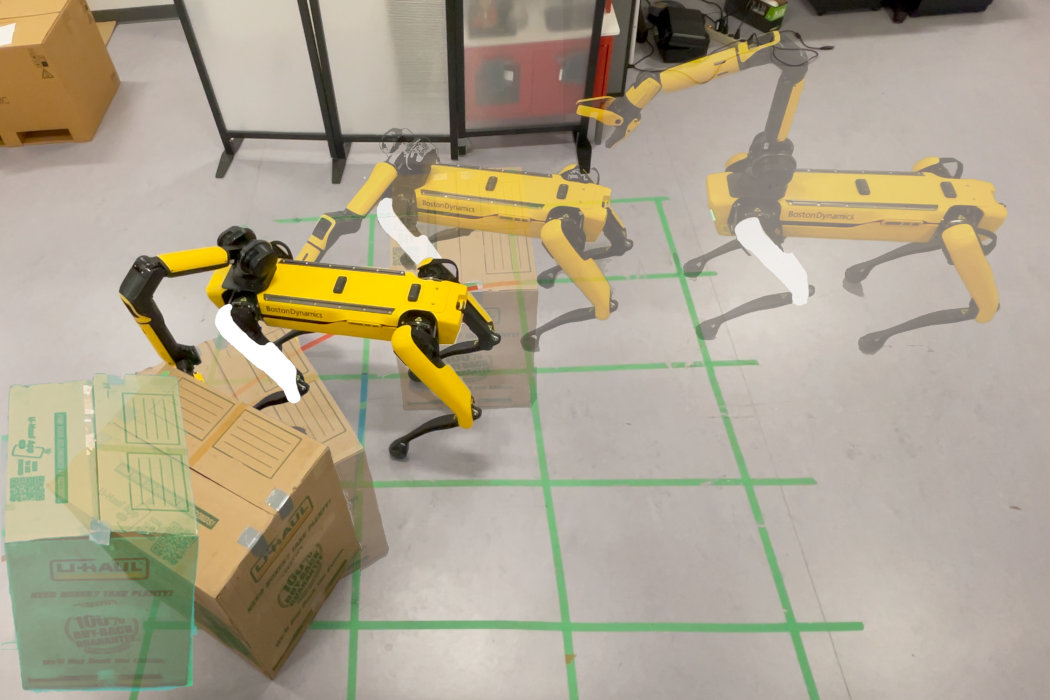
\includegraphics[width=\textwidth]{figures/chapter5/12pt5kg-Policy.jpg}
        \caption{Policy, 12.5\,kg}
    \end{subfigure}
    \hfill
    \begin{subfigure}[t]{0.48\textwidth}
        \centering
        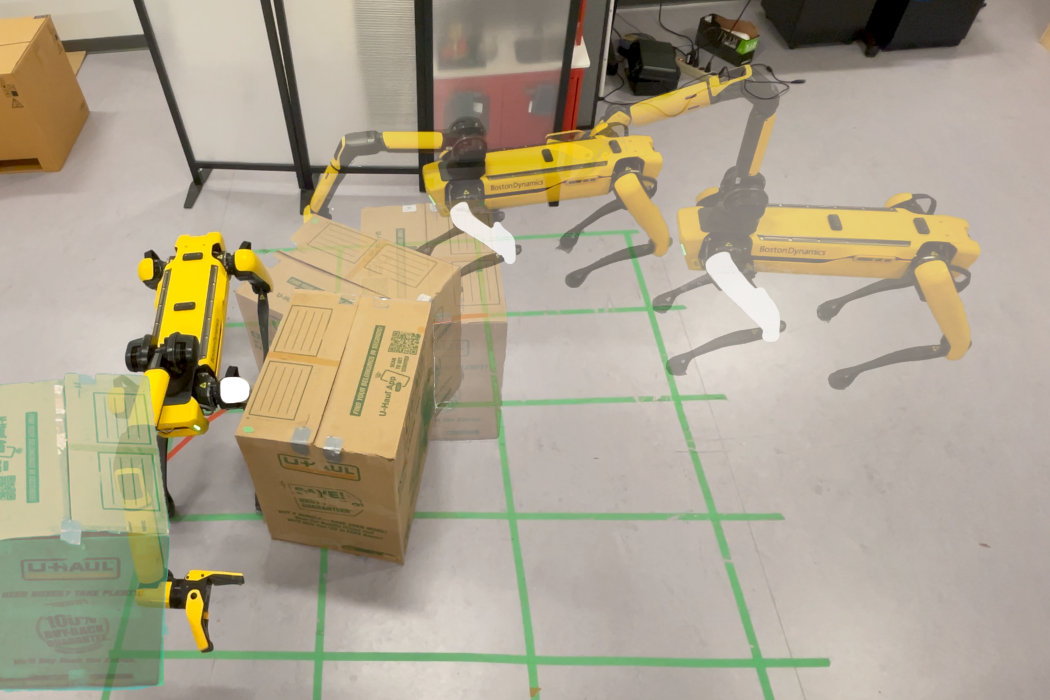
\includegraphics[width=\textwidth]{figures/chapter5/12pt5kg-baseline.jpg}
        \caption{Baseline, 12.5\,kg}
    \end{subfigure}
    \caption{Chronophotographic composites of real-world box transport on the Boston Dynamics Spot. Top row: proposed force-based policy under $8.8$~kg (a) and $12.5$~kg (c) payloads, showing consistent trajectory tracking. Bottom row: kinematic baseline under the same conditions (b, d), showing frequent deviation and failure to reach the goal.}
    \label{fig:pho_realworld}
\end{figure}
\subsubsection{Real-World Experiments}

The learned policy was deployed zero-shot on a Boston Dynamics Spot mobile manipulator without retraining. Only impedance gains ($K_\text{eff} = 300$, $\zeta = 45$) were tuned to ensure stable, non-oscillatory contact. Experiments were conducted with two unknown payload conditions ($8.8$~kg and $12.5$~kg), with 10 trials per condition for both the proposed policy and a kinematic trajectory-following baseline, for a total of 40 real-world trials.

\paragraph{Reactive force estimation.} Prior to each trial, the robot performs the impedance-based probing routine to estimate $z$. The estimated reactive forces are $26.18 \pm 2.07$~N for the $8.8$~kg object and $41.74 \pm 2.20$~N for the $12.5$~kg object, consistent with expected increases in contact resistance and showing low variance within each condition.

\paragraph{Execution performance.} The proposed policy successfully transported the object to the target endpoint in 17 out of 20 attempts across both payload conditions. The trajectory-following baseline did not reach the goal region in any trial (0/20). This consistent separation across repeated trials indicates that the performance difference is not attributable to stochastic variation in execution.

\paragraph{Qualitative observations.} The baseline controller frequently deviated from the intended trajectory and struggled to maintain sustained contact, particularly under the heavier payload. The force-based policy maintained consistent pushing behavior across both masses and completed the curved transport task in the majority of trials. The dominant failure mode was contact loss caused by slip at the gripper--object interface, which was partially mitigated by a brief zero-stiffness impedance recovery step.